%Para slide em "Wide-Screen" usar:
\documentclass[aspectratio=169]{beamer} 

%Para slide "quadrado" usar:
%\documentclass{beamer} 



\usepackage{tikz}

%\setbeamercolor{block title}{bg=red!30,fg=black}

\usepackage[most]{tcolorbox}



\usepackage{booktabs} 
\usepackage{subcaption}

%\usetheme{Ufg}
%\usetheme{Oxygen}
\usepackage{thumbpdf}
\usepackage{wasysym}
\usepackage{ucs}
\usepackage[utf8]{inputenc}
\usepackage{pgf,pgfarrows,pgfnodes,pgfautomata,pgfheaps,pgfshade}
\usepackage{verbatim}
\usepackage{tikzsymbols}

\usepackage{ragged2e} % maneja la alineación del documento
\usepackage[spanish]{babel} % Títulos en español
\usepackage[utf8]{inputenc}
%\usepackage[latin1]{inputenc} % Caracteres con acentos.
\usepackage{graphicx} % Soporte para gráficos
\usepackage[none]{hyphenat} % indica a LaTeX que no debe hacer partición de palabras
\usepackage[T1]{fontenc} % manejo de fuentes
\usepackage{array}
\usepackage{amsmath}
\usepackage{amssymb}
\usepackage{float}
%\usepackage{ra  gged2e}
\usepackage [all]{xy}
\usepackage{lmodern}
\usepackage{multirow}
\usepackage{multicol}
\usepackage{tikz}
\usepackage{listings}
\usepackage{shapepar}






%Elaborado por Mateus Moro Lumertz

\author{mateuslumertz}
\definecolor{cor1}{RGB}{0,100,166}
\definecolor{cor2}{RGB}{100,195,213}
\definecolor{cor5}{RGB}{150,203,226}
\definecolor{cor3}{RGB}{30,130,186}
\definecolor{cor4}{RGB}{40,185,218}
\definecolor{preto}{RGB}{0,0,0}
\definecolor{branco}{RGB}{255,255,255}
% Configuração das Cores
\setbeamercolor{paleta1}{fg=cor1,bg=white}
\setbeamercolor{paleta2}{fg=cor1,bg=white}
\setbeamercolor{estrutura}{fg=cor1,bg=white}
\setbeamercolor{titulo_rodape}{fg=black,bg=white}
\setbeamercolor{data_rodape}{fg=gray,bg=white}
\setbeamercolor{frametitle}{fg=branco,bg=cor1}
\setbeamertemplate{caption}[numbered]

\definecolor{block-gray}{gray}{0.85}
\newtcolorbox{blockquote}{colback=block-gray,grow to right by=-1mm,grow to left by=-1mm,boxrule=0pt,boxsep=0pt,breakable}


% Modelo do rodapé
\defbeamertemplate*{footline}{mytheme}{%
  \leavevmode%
  \hbox{\begin{beamercolorbox}[wd=.5\paperwidth,ht=2.5ex,dp=1.125ex,leftskip=.3cm,rightskip=.3cm]{titulo_rodape}%
    \makebox[2em][l]{{\usebeamerfont{titulo_rodape}\textcolor{cor1}{\insertframenumber}}}%
    {\usebeamercolor{titulo_rodape}\insertshorttitle}
  \end{beamercolorbox}%
  \begin{beamercolorbox}[wd=.2\paperwidth,ht=2.5ex,dp=1.125ex,leftskip=.3cm,rightskip=.3cm]{data_rodape}%
    \usebeamerfont{data_rodape}\insertshortdate%
  \end{beamercolorbox}%
  \begin{beamercolorbox}[wd=.3\paperwidth,ht=2.5ex,dp=1.125ex,leftskip=.3cm,rightskip=.3cm,right]{titulo_rodape}%
    \includegraphics[width=.8\paperwidth,height=12ex,keepaspectratio]{logo.png}\hspace*{2em}%
  \end{beamercolorbox}}%
  \vskip0pt%
}

% Slide de Título
\defbeamertemplate*{title page}{mytheme}[1][]
{%
  \begin{tikzpicture}[remember picture,overlay]
    \filldraw[cor1]
    (current page.north west) --
    ([yshift=-12cm]current page.north west) --
    ([xshift=-4cm,yshift=-12cm]current page.north east) {[rounded corners=15pt]--
    ([xshift=-4cm,yshift=3cm]current page.south east)} --
    ([yshift=3cm]current page.south west) --
    (current page.south west) --
    (current page.south east) --
    (current page.north east) -- cycle
    ;
  \filldraw[branco]
    (current page.north west) --
    ([yshift=-2.15cm]current page.north west) --
    ([xshift=-3cm,yshift=-2.15cm]current page.north east) {[rounded corners=15pt]--
    ([xshift=-3cm,yshift=3cm]current page.south east)} --
    ([yshift=3cm]current page.south west) --
    (current page.south west) --
    (current page.south east) --
    (current page.north east) -- cycle
    ;
    \filldraw[cor2]
    ([xshift=-0.25cm,yshift=3cm]current page.south east)--
    ([xshift=-2.75cm,yshift=3cm]current page.south east)--
    ([xshift=-2.75cm,yshift=3.85cm]current page.south east)--
    ([xshift=-0.25cm,yshift=3.85cm]current page.south east)-- cycle
    ;
    \filldraw[cor3]
    ([xshift=-0.25cm,yshift=4cm]current page.south east)--
    ([xshift=-2.75cm,yshift=4cm]current page.south east)--
    ([xshift=-2.75cm,yshift=4.85cm]current page.south east)--
    ([xshift=-0.25cm,yshift=4.85cm]current page.south east)-- cycle
    ;
    \filldraw[cor4]
    ([xshift=-0.25cm,yshift=5cm]current page.south east)--
    ([xshift=-2.75cm,yshift=5cm]current page.south east)--
    ([xshift=-2.75cm,yshift=5.85cm]current page.south east)--
    ([xshift=-0.25cm,yshift=5.85cm]current page.south east)-- cycle
    ;
    \filldraw[cor5]
    ([xshift=-0.25cm,yshift=6cm]current page.south east)--
    ([xshift=-2.75cm,yshift=6cm]current page.south east)--
    ([xshift=-2.75cm,yshift=6.85cm]current page.south east)--
    ([xshift=-0.25cm,yshift=6.85cm]current page.south east)-- cycle
    ;
  \node[text=branco,anchor=south west,font=\sffamily\LARGE,text width=.68\paperwidth] 
  at ([xshift=10pt,yshift=-0.5cm]current page.west)
  (title)
  {\raggedright\inserttitle};  
  
  \node[text=cor1,anchor=south west,font=\sffamily\small,text width=.75\paperwidth] 
  at ([xshift=10pt,yshift=3.6cm]current page.west)
  (title)
  {\raggedright Universidad del Valle, Facultad de Ingeniería};  
  
  
  % \node[anchor=west]
  %at ([xshift=10.1cm,yshift=8.5cm]current page.south west)
  %{\includegraphics[height=1.5cm]{logo.png}};
  
  \node[anchor=east]
  at ([xshift=-0.15cm,yshift=-1cm]current page.north east)
  {\includegraphics[width=2.5cm]{logo.png}};
  
  \node[text=preto,font=\large\sffamily,anchor=south west]
  at (0,-5)
  (date)
  {\insertdate};
  \node[text=preto,font=\large\sffamily,anchor=south west]
  at (0,-3.8)
  (author)
  {\insertauthor};
  \node[text=preto,font=\large\sffamily,anchor=south west]
  at (0,-4.5)
  (institute)
  {\insertinstitute};
  \end{tikzpicture}%
}

% remove navigation symbols
\setbeamertemplate{navigation symbols}{}


% definition of the itemize templates
\setbeamertemplate{itemize item}[circle]
\setbeamercolor{itemize item}{fg=cor3,bg=white}
\setbeamercolor{itemize subitem}{fg=cor4,bg=white}
\setbeamercolor{itemize subsubitem}{fg=cor2,bg=white}



\title[Maestría en Analítica e Inteligencia de Negocios]{Value at Risk (VaR)}
\author{Orlando Joaqui Barandica}
\institute{Maestría en Analítica e Inteligencia de Negocios}
\date{2021}



\sloppy % Indica a LaTex que debe minimizar el corte de las palabras para pasar de una línea a otra
\justifying % justificar todo el documento



\begin{document}

\begin{frame}[plain]
\maketitle
\end{frame}



\begin{frame}
  \frametitle{Contenido}
  \tableofcontents[hidesubsections]
\end{frame}



%%%%%%%%%%%%%%%%%%%%%%%%%%%%%%%%%%%%%%%%%%%%%%%%%%%%%%%%%%%%%%%%%%%%%%%
%Slide 1
\section{Introducción}
\begin{frame}
\frametitle{Value at Risk}
\framesubtitle{Introducción}


El Valor en Riesgo (VaR) es una de las medidas utilizadas para evaluar el riesgo de una determinada posición o cartera de activos financieros.\\

\vspace{4mm}
La definición del VaR puede hacerse en términos de \textcolor{teal}{rentabilidades} o en términos de \textcolor{orange}{Pérdidas y Ganancias} P\&L (términos nominales); la definición también depende de que se aplique a una posición larga (comprada), como es habitual, o a una posición corta (vendida) en un activo financiero


\end{frame}



%%%%%%%%%%%%%%%%%%%%%%%%%%%%%%%%%%%%%%%%%%%%%%%%%%%%%%%%%%%%%%%%%%%%%%


\begin{frame}
\frametitle{Value at Risk}
\framesubtitle{Introducción}



\begin{columns}
\begin{column}{0.5\textwidth}


\begin{center}
\textcolor{orange}{El VaR responde entonces a la pregunta:}
\end{center}

\vspace{4mm}

\textit{¿Cuál es la caída o pérdida que se podría sufrir en condiciones normales de mercado en un intervalo de tiempo y con cierto nivel de probabilidad o de confianza?
}



\end{column}
\begin{column}{0.5\textwidth}  %%<--- here
\begin{figure}[h!]
\begin{center}
    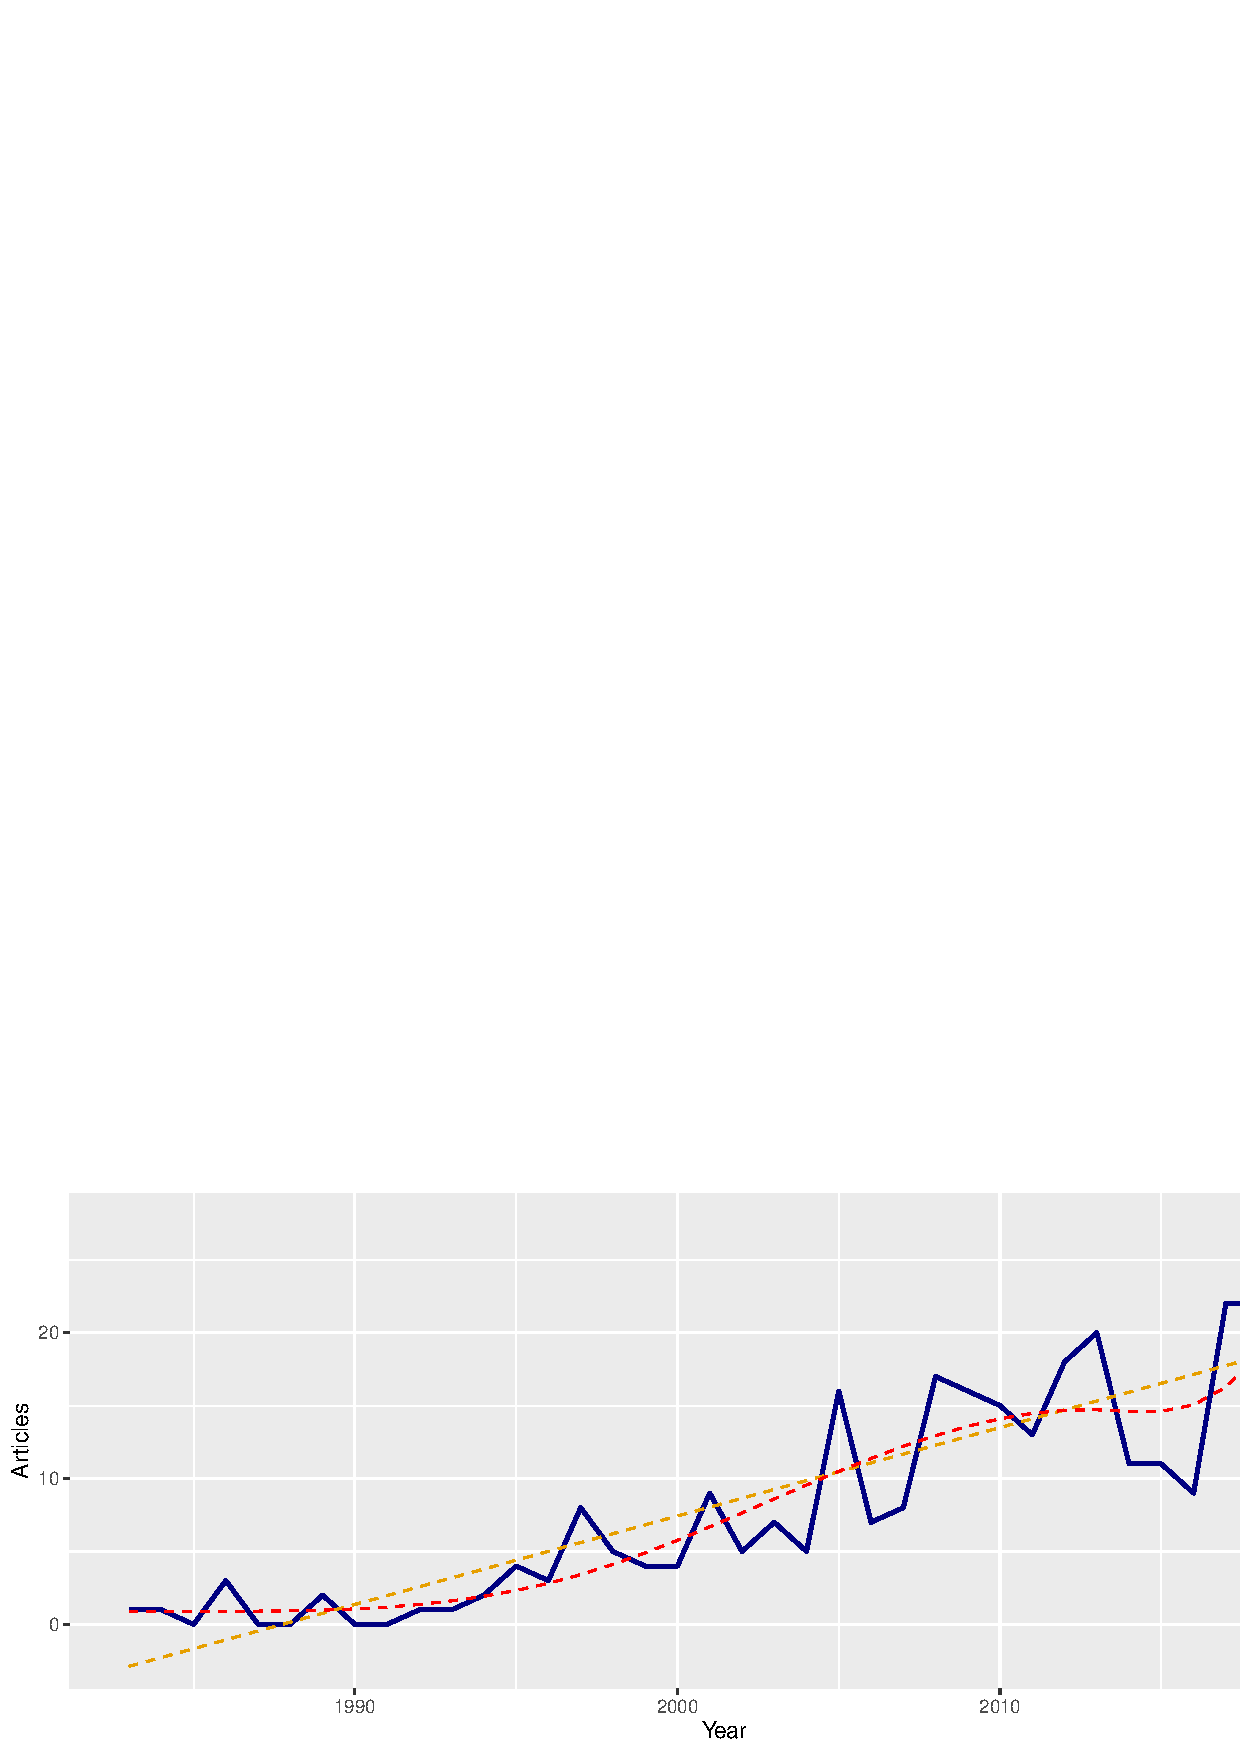
\includegraphics[width=1\textwidth]{Imagen1.JPEG}
\end{center}
\end{figure}
\end{column}
\end{columns}




\end{frame}



%%%%%%%%%%%%%%%%%%%%%%%%%%%%%%%%%%%%%%%%%%%%%%%%%%%%%%%%%%%%%%%%%%%%%%%





\begin{frame}
\frametitle{Value at Risk}
\framesubtitle{Introducción}



\begin{columns}
\begin{column}{0.5\textwidth}

\vspace{10mm}

\begin{center}
Es decir, indica la probabilidad (normalmente 1\% o 5\%) de sufrir una determinada pérdida durante un periodo de tiempo (normalmente 1 día, 1 semana o 1 mes).
\end{center}

\vspace{4mm}

\end{column}
\begin{column}{0.5\textwidth}  %%<--- here

\begin{center}
\textcolor{orange}{Una interpretación equivalente es:}\\
\end{center}

\vspace{2mm}

\begin{itemize}
\item Con probabilidad 1-$\alpha$ el propietario de dicha posición experimentará una pérdida no superior al VaR.
\end{itemize}

\end{column}
\end{columns}


\pause
\begin{center}
\textcolor{teal}{\textbf{Ej:} una entidad financiera podría considerar que el VaR diario de una cartera operativa es de 50 millones de euros, con un nivel de confianza del 90\%. Esto quiere decir que solamente hay 1 posibilidad en 10, en condiciones normales de mercado, de que haya una pérdida superior a los 50 millones de euros.}
\end{center}



\end{frame}



%%%%%%%%%%%%%%%%%%%%%%%%%%%%%%%%%%%%%%%%%%%%%%%%%%%%%%%%%%%%%%%%%%%%%%%




\begin{frame}
\frametitle{Value at Risk}
\framesubtitle{Introducción}



\begin{columns}
\begin{column}{0.5\textwidth}

\begin{figure}[h!]
\begin{center}
    \includegraphics[width=1\textwidth]{Imagen2.JPEG}
\end{center}
\end{figure}



\end{column}
\begin{column}{0.5\textwidth}  %%<--- here

Por consiguiente, el VaR no es sino un determinado percentil de la distribución de probabilidad prevista para las variaciones en el valor de mercado de la cartera en el horizonte de tiempo escogido.

\end{column}
\end{columns}




\end{frame}



%%%%%%%%%%%%%%%%%%%%%%%%%%%%%%%%%%%%%%%%%%%%%%%%%%%%%%%%%%%%%%%%%%%%%%%



\section{Métodos}
\begin{frame}
\frametitle{Cálculo del VaR}
\framesubtitle{Métodos}



\begin{itemize}
\item \textbf{VaR Histórico, No Paramétrico:} se encuentra el $\alpha$ percentil de la distribución histórica de los datos.

\vspace{4mm}

\item \textbf{VaR Paramétrico:} se calcula el VaR con base en un modelo que describe su función de densidad de las pérdidas. La cual debe ser estimada.

\begin{itemize}
\item VaR suponiendo que las pérdidas siguen una distribución Gaussiana no condicional.

\item VaR modelando los valores futuros de la media y la varianza condicionales.

\item VaR por simulación de Montecarlo (estimando la función multivariada que describe los datos, por ejemplo mediante cópulas)
\end{itemize} 


\end{itemize}



\end{frame}



%%%%%%%%%%%%%%%%%%%%%%%%%%%%%%%%%%%%%%%%%%%%%%%%%%%%%%%%%%%%%%%%%%%%%%%




\subsection{Método gaussiano}
\begin{frame}
\frametitle{Método paramétrico}
\framesubtitle{Distribución gaussiana}



\begin{columns}
\begin{column}{0.5\textwidth}

{\small
\begin{itemize}
\item Suponemos que la distribución de las rentabilidades de los factores sigue una distribución Normal multivariante y la cartera es función lineal de los factores.

\item Su ventaja es que es tratable analíticamente, pero solo se puede generalizar a una pocas formas paramétricas, como la Normal, la t-Student, o mixturas de Normales o de t-Student.

\item La regla de la raiz cuadrada en la extrapolación de la varianza no es válida.
\end{itemize}
}


\pause

\end{column}
\begin{column}{0.5\textwidth}  %%<--- here

{\small
\begin{center}
\textcolor{teal}{Como $\alpha$ es un valor reducido: 5\%, 1\% o 0.01\%, entonces $R^*$ será una rentabilidad negativa, y el VaR se proporciona cambiando el signo.}
\end{center}

\begin{equation}
VaR = -R^* \textcolor{orange}{\Rightarrow} \alpha = P(R<R^*) = \Phi\left( \frac{R^*-\mu_R}{\sigma_R} \right) \nonumber
\end{equation}

\begin{equation}
\textcolor{orange}{VaR_{(1-\alpha)} = \Phi^{-1}(1-\alpha) \sigma_R - \mu_R}  \nonumber
\end{equation}

}

\end{column}
\end{columns}


\end{frame}



%%%%%%%%%%%%%%%%%%%%%%%%%%%%%%%%%%%%%%%%%%%%%%%%%%%%%%%%%%%%%%%%%%%%%%%



\begin{frame}
\frametitle{Método paramétrico}
\framesubtitle{Distribución gaussiana}



\begin{itemize}
\item \textbf{Método de normalidad estático}

\begin{equation}
\textcolor{orange}{VaR_{(1-\alpha)} = \Phi^{-1}(1-\alpha) \sigma_R - \mu_R}  \nonumber
\end{equation}


\vspace{4mm}

\item \textbf{Método de normalidad condicional}


\begin{equation}
\textcolor{orange}{VaR_{(1-\alpha),t+1} = \Phi^{-1}(1-\alpha) \sigma_{R,t+1} - \mu_{R,t+1}}  \nonumber
\end{equation}

\begin{itemize}
\item Estimación de $\mu_{t+1}$: Modelos ARIMA de series de tiempo
\item Estimación de $\sigma_{t+1}$: Modelos de varianza condicional:

\begin{itemize}
\item Modelos GARCH: como un ARMA sobre la varianza con algunas restricciones.
\item Modelos de Volatilidad Estocástica: una versión más general de los GARCH.
\end{itemize}
\end{itemize}

\end{itemize}



\end{frame}



%%%%%%%%%%%%%%%%%%%%%%%%%%%%%%%%%%%%%%%%%%%%%%%%%%%%%%%%%%%%%%%%%%%%%%%





\subsection{Histórico}
\begin{frame}
\frametitle{Método no paramétrico}
\framesubtitle{VaR histórico}



\begin{columns}
\begin{column}{0.5\textwidth}

{\small
\begin{itemize}
\item No precisa hacer supuestos acerca de la forma paramétrica de la distribución de rentabilidades de los factores de riesgo o de la cartera.

\item No está limitado a carteras en las que los pagos tienen una estructura
lineal.

\item El método histórico debe utilizarse solo para el cálculo del VaR a un
horizonte de muy pocos días.

\end{itemize}
}



\end{column}
\begin{column}{0.5\textwidth}  %%<--- here

\begin{equation}
\textcolor{teal}{VaR_{(1-\alpha)} = q_{(1-\alpha)(R)}}  \nonumber
\end{equation}

\end{column}
\end{columns}




\end{frame}



%%%%%%%%%%%%%%%%%%%%%%%%%%%%%%%%%%%%%%%%%%%%%%%%%%%%%%%%%%%%%%%%%%%%%%%





\subsection{Simulación de Montecarlo}
\begin{frame}
\frametitle{Método paramétrico}
\framesubtitle{Simulación de MonteCarlo}



\begin{itemize}
\item \textbf{Método de simulación Montecarlo - estático}

\begin{equation}
\textcolor{orange}{VaR_{(1-\alpha)} = \sigma_R(-q_{(1-\alpha)}(Z))  - \mu_R, \quad \quad Z\sim N(0,1)}  \nonumber
\end{equation}


\vspace{4mm}

\item \textbf{Método de simulación Montecarlo - dinámico}


\begin{equation}
\textcolor{orange}{VaR_{(1-\alpha)} = \sigma_{R,t+1}(-q_{(1-\alpha)}(Z))  - \mu_{R,t+1}, \quad \quad Z\sim N(0,1)}  \nonumber
\end{equation}

\end{itemize}



\end{frame}



%%%%%%%%%%%%%%%%%%%%%%%%%%%%%%%%%%%%%%%%%%%%%%%%%%%%%%%%%%%%%%%%%%%%%%%





\section{Expected Shortfall}
\begin{frame}
\frametitle{Limitaciones}
\framesubtitle{VaR}


Como se puede observar existen diversas metodologías, con diferentes niveles de precisión, para estimar el Valor en Riesgo. No obstante, todas estas metodologías presentan limitaciones generales, que caracterizan la técnica del VaR y que por ende son imposibles de evitar sin recurrir a otras herramientas.


\begin{block}{}
\begin{itemize}
\item Dice muy poco sobre los casos en las colas (pérdidas extremas).
\item Puede crear estructuras perversas de incentivos (porque no se
conoce la magnitud de las pérdidas que exceden las colas).

\end{itemize}
\end{block}


\end{frame}



%%%%%%%%%%%%%%%%%%%%%%%%%%%%%%%%%%%%%%%%%%%%%%%%%%%%%%%%%%%%%%%%%%%%%%%



\begin{frame}
\frametitle{Expected Shortfall}
\framesubtitle{CVaR}


\begin{columns}
\begin{column}{0.5\textwidth}

Mientras que el \textcolor{teal}{VaR estima lo máximo que se puede esperar perder} si un evento de pérdidas extremas no ocurre, es decir, la peor pérdida esperada en caso de una relativa regularidad financiera, el \textcolor{orange}{ES (Expected Shortfall) indica cuánto se espera perder si un evento extremo efectivamente ocurre} (más allá del nivel de confianza del VaR, en las colas de la distribución).


\begin{equation}
ES = E[R / ( R < VaR )] \nonumber
\end{equation}



\end{column}
\begin{column}{0.5\textwidth}  %%<--- here

\begin{figure}[h!]
\begin{center}
    \includegraphics[width=1\textwidth]{Imagen3.JPEG}
\end{center}
\end{figure}

\end{column}
\end{columns}






\end{frame}



%%%%%%%%%%%%%%%%%%%%%%%%%%%%%%%%%%%%%%%%%%%%%%%%%%%%%%%%%%%%%%%%%%%%%%%




%%%%%%%%%%%%%%%%%%%%%%%%%%%%%%%%%%%%%%%%%%%%%%%%%%%%%%%%%%%%%%%%%%%%%%%



\begin{frame}
\frametitle{}
\framesubtitle{}

  \vspace{2cm}
  {\huge Preguntas?}


\vspace{2.5cm}

\begin{flushright}
\textcolor{orange}{  \usebeamerfont*{frametitle}Gracias!!,}
\end{flushright}

  
  \begin{flushright}
    Jr.
    
   \structure{\footnotesize{orlando.joaqui@correounivalle.edu.co}}
  \end{flushright}


\end{frame}



%%%%%%%%%%%%%%%%%%%%%%%%%%%%%%%%%%%%%%%%%%%%%%%%%%%%%%%%%%%%%%%%%%%%%%%


%%%%%%%%%%%%%%%%%%%%%%%%%%%%%%%%%%%%%%%%%%%%%%%%%%%%%%%%%%%%%%%%%%%%%%%
%Slide 3



\end{document}